\chapter{研究设计}

\section{资料来源与纳入原则}

本示例完全基于公开资料，不包含真实病历、访谈录音、内部审稿件或未公开正文。资料来源包括：主流媒体报道、节目档期、公开号运营记录、杂志封面时间线以及平台公开的互动数据。纳入标准强调三个条件：事件时间明确、信息来源可追溯、且能够对应到职业阶段的变化。

\section{分析框架}

本研究采用“阶段划分-事件编码-韧性评分”三层框架。阶段划分解决“什么时候发生转折”，事件编码回答“转折由什么驱动”，韧性评分则用于比较不同阶段的恢复效率与叙事掌控度。

\begin{table}[H]
  \centering
  \caption{公开案例研究的核心变量}
  \label{tab:smu-variables}
  \begin{tabularx}{0.92\textwidth}{>{\raggedright\arraybackslash}p{0.18\textwidth} >{\raggedright\arraybackslash}p{0.26\textwidth} X}
    \toprule
    变量层级 & 变量名称 & 含义说明 \\
    \midrule
    阶段层 & 职业阶段 & 出道、扩张、危机、重启四个时间段 \\
    事件层 & 平台迁移 & 是否进入新的主要传播平台 \\
    事件层 & 角色变化 & 是否出现从模特到演员、综艺或创作者的角色扩展 \\
    结果层 & 韧性得分 & 对叙事控制、公众接受度与持续产出的综合评分 \\
    \bottomrule
  \end{tabularx}
\end{table}

\section{编码流程}

研究首先按时间顺序建立事件表，再根据事件性质进行双重编码：一类编码关注“平台变化”，另一类编码关注“叙事变化”。当同一时间段既有平台变化又有叙事变化时，采用联合标记。这样的设计可以把“职业行为”与“公众反馈”放在同一分析面板中。

\begin{longtable}{p{0.16\textwidth}p{0.20\textwidth}p{0.20\textwidth}p{0.28\textwidth}}
  \caption{阶段化编码示例表}\label{tab:smu-longtable}\\
  \toprule
  阶段 & 关键事件 & 主要平台 & 解释性备注 \\
  \midrule
  \endfirsthead
  \toprule
  阶段 & 关键事件 & 主要平台 & 解释性备注 \\
  \midrule
  \endhead
  出道期 & 模特比赛获奖 & 时尚杂志 & 通过单一平台建立早期识别度 \\
  扩张期 & 转入影视与综艺 & 电视与访谈节目 & 实现受众外延扩张 \\
  危机期 & 私生活争议暴露 & 社交媒体与新闻平台 & 可控叙事迅速减弱，公众评价波动扩大 \\
  修复期 & 低频公开表达 & 传统媒体与品牌合作 & 以有限曝光维持可见度，减少额外争议 \\
  重启期 & 开设个人频道 & 视频平台 & 重新掌握发布节奏与内容框架 \\
  \bottomrule
\end{longtable}

\section{媒介能力差异}

\begin{figure}[H]
  \centering
  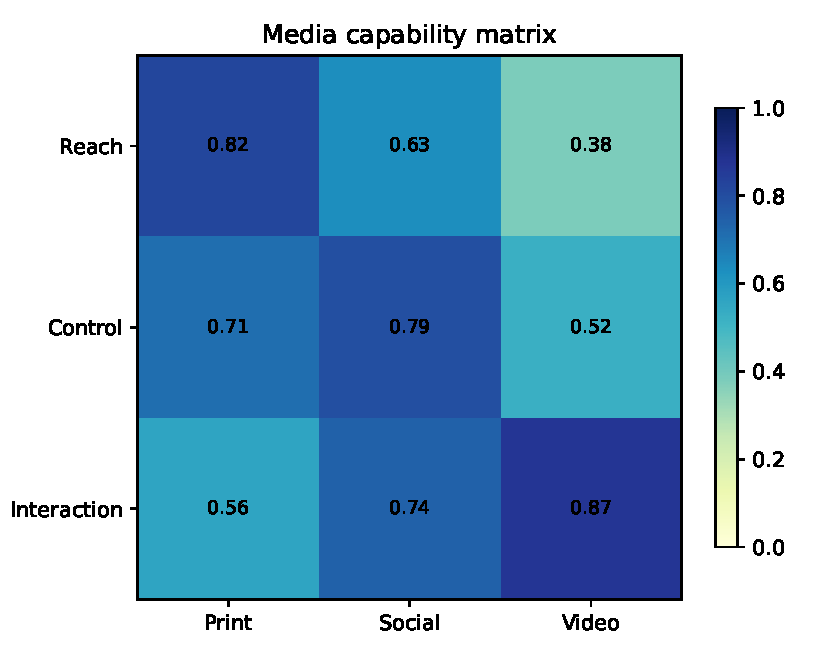
\includegraphics[width=0.72\textwidth]{assets/demo/media-matrix.pdf}
  \caption{不同平台的能力矩阵}
  \label{fig:smu-matrix}
\end{figure}

\figref{fig:smu-matrix} 展示了三类平台在可达性、互动性与自主性上的差异。这个示意图并不声称反映真实行业测量值，而是为模板用户演示“图+文解释+交叉引用”的常见写法。
